\documentclass[a4paper,oneside,12pt]{report}
% Package yang diperlukan
\usepackage{graphicx}      % Untuk memasukkan gambar
\usepackage{geometry}      % Untuk mengatur margin halaman
\usepackage{listings}      % Untuk menampilkan blok kode
\usepackage{xcolor}        % Untuk menggunakan warna
\usepackage{float}         % Untuk kontrol penempatan float (seperti gambar)
\usepackage{hyperref}      % Untuk membuat hyperlink (URL, referensi)
\usepackage{natbib}        % Untuk citation dengan \cite{} yang clickable
\usepackage{indentfirst}   % Untuk memberi indentasi pada paragraf pertama setiap seksi
\usepackage{url}           % Untuk format URL
\usepackage{fancyhdr}      % Untuk kustomisasi header dan footer
\usepackage{tocloft}       % Untuk kustomisasi Daftar Isi
\usepackage{bookmark}      % Untuk manajemen bookmark PDF yang lebih baik

%======================================================================
% PENGATURAN GEOMETRI HALAMAN
%======================================================================
% Margin umum untuk isi laporan
\geometry{left=3cm, right=2.5cm, top=2cm, bottom=2.5cm}
\sloppy

%======================================================================
% PENGATURAN WARNA UNTUK BLOK KODE
%======================================================================
\definecolor{codegreen}{rgb}{0,0.6,0}
\definecolor{codegray}{rgb}{0.5,0.5,0.5}
\definecolor{codepurple}{rgb}{0.58,0,0.82}
\definecolor{backcolour}{rgb}{0.95,0.95,0.92}
\definecolor{darkblue}{rgb}{0,0,0.6}

%======================================================================
% PENGATURAN BLOK KODE (LISTINGS)
%======================================================================
% Gaya umum untuk semua blok kode
\lstdefinestyle{commonstyle}{
    backgroundcolor=\color{backcolour}, 
    breakatwhitespace=false, 
    breaklines=true, 
    captionpos=b, 
    keepspaces=true,
    numbers=left, 
    numbersep=5pt, 
    showspaces=false, 
    showstringspaces=false,
    showtabs=false, 
    tabsize=2, 
    frame=single,
    basicstyle=\ttfamily\footnotesize,
    numberstyle=\tiny\color{codegray},
    columns=flexible,
    postbreak=\mbox{\textcolor{red}{$\hookrightarrow$}\space},
    breakindent=0pt,
    breakautoindent=false
}

% Gaya khusus untuk HTML
\lstdefinestyle{htmlstyle}{
    style=commonstyle,
    language=HTML,
    commentstyle=\color{codegreen},
    keywordstyle=\color{codepurple},
    stringstyle=\color{codegreen},
    basicstyle=\ttfamily\scriptsize
}

% Gaya khusus untuk CSS
\lstdefinestyle{cssstyle}{
    style=commonstyle,
    commentstyle=\color{codegreen},
    keywordstyle=\color{darkblue},
    stringstyle=\color{codepurple},
    emph={color, background, font, margin, padding, border, display, position, width, height},
    emphstyle=\color{darkblue},
    basicstyle=\ttfamily\scriptsize
}

% Gaya khusus untuk Python
\lstdefinestyle{pythonstyle}{
    style=commonstyle,
    language=Python,
    commentstyle=\color{codegreen},
    keywordstyle=\color{darkblue},
    stringstyle=\color{codepurple},
    emph={import,from,class,def,for,while,if,else,elif,try,except,finally},
    emphstyle=\color{darkblue}
}

% Gaya khusus untuk SQL
\lstdefinestyle{sqlstyle}{
    style=commonstyle,
    language=SQL,
    commentstyle=\color{codegreen},
    keywordstyle=\color{darkblue},
    stringstyle=\color{codepurple},
    emph={SELECT,FROM,WHERE,INSERT,UPDATE,DELETE,CREATE,DROP},
    emphstyle=\color{darkblue}
}

% Gaya khusus untuk JavaScript
\lstdefinestyle{javascriptstyle}{
    style=commonstyle,
    language=JavaScript,
    commentstyle=\color{codegreen},
    keywordstyle=\color{darkblue},
    stringstyle=\color{codepurple},
    emph={function,var,let,const,return,if,for,while,do,else,switch,case},
    emphstyle=\color{darkblue}
}

% Gaya khusus untuk Java
\lstdefinestyle{javastyle}{
    style=commonstyle,
    language=Java,
    commentstyle=\color{codegreen},
    keywordstyle=\color{darkblue}\bfseries,
    stringstyle=\color{codepurple},
    emph={@Test,@Mock,@InjectMocks,@ExtendWith},
    emphstyle=\color{codepurple}
}

%======================================================================
% PENGATURAN LAIN-LAIN
%======================================================================

% Mengganti nama default "Figure" menjadi "Gambar"
\renewcommand{\figurename}{Gambar}
\renewcommand{\thefigure}{\arabic{figure}}

% Pengaturan Hyperlink
\hypersetup{
    colorlinks=true, 
    linkcolor=black, 
    filecolor=black, 
    urlcolor=black,
    citecolor=blue,
    pdftitle={Laporan Praktikum}, 
    pdfpagemode=FullScreen, 
    breaklinks=true
}

% Pengaturan citation style
\bibliographystyle{plain}

% Pengaturan Header & Footer (nomor halaman di tengah bawah)
\pagestyle{fancy}
\fancyhf{}
\fancyfoot[C]{\thepage}
\renewcommand{\headrulewidth}{0pt}

\fancypagestyle{plain}{
    \fancyhf{}
    \fancyfoot[C]{\thepage}
    \renewcommand{\headrulewidth}{0pt}
}

%======================================================================
% PENGATURAN STRUKTUR BAB DAN DAFTAR ISI
%======================================================================
\renewcommand{\contentsname}{Daftar Isi}
\renewcommand{\bibname}{Daftar Pustaka}

% Menghilangkan nomor bab tetapi mempertahankan penomoran seksi
\renewcommand{\thechapter}{}
\renewcommand{\chaptername}{}

% Format penomoran seksi menjadi [nomor bab].[nomor seksi]
\renewcommand{\thesection}{\arabic{chapter}.\arabic{section}}
\renewcommand{\thesubsection}{\thesection.\arabic{subsection}}

\setcounter{secnumdepth}{3}
\setcounter{tocdepth}{2}

% Format Daftar Isi (TOC)
\renewcommand{\cftchapdotsep}{\cftdotsep}
\renewcommand{\cftchapleader}{\cftdotfill{\cftchapdotsep}}
\setlength{\cftchapindent}{0em}
\setlength{\cftsecindent}{2em}
\setlength{\cftsubsecindent}{4em}
\setlength{\cftchapnumwidth}{0em}
\setlength{\cftsecnumwidth}{2.5em}
\setlength{\cftsubsecnumwidth}{3.2em}
\renewcommand{\cftchappresnum}{}
\renewcommand{\cftchapaftersnum}{}

% Perintah kustom untuk membuat judul bab di TOC menjadi tebal
\newcommand{\tocboldsection}[1]{%
  \protect\renewcommand{\protect\cftchapfont}{\protect\bfseries}%
  #1%
  \protect\renewcommand{\protect\cftchapfont}{}%
}

%======================================================================
% AWAL DOKUMEN
%======================================================================
\begin{document}

% Halaman Judul
\newgeometry{left=3cm, right=2.5cm, top=2.5cm, bottom=3cm}
\begin{titlepage}
\begin{center}
\vspace*{0.5cm}
{\large \textbf{\MakeUppercase{Laporan Praktikum}}} \\[0.4cm]
{\large \textbf{\MakeUppercase{PRAKTIKUM PENGUJIAN PERANGKAT LUNAK}}} \\[0.4cm]
{\large \textbf{\MakeUppercase{Pertemuan 7}}} \\[0.4cm]
{\large \textbf{\MakeUppercase{AUTOMATION TESTING}}} \\[1.5cm]


\includegraphics[height=7cm]{lambang ugm.png} \\[1cm]

{\normalsize \textbf{Disusun oleh:}} \\[0.4cm]
\begin{tabular}{@{}l l @{}}
  \textbf{Nama}           & : Januarsyah Akbar \\
  \textbf{NIM}            & : 24/535846/SV/24314 \\
  \textbf{Kelas}          & : PL4B2 \\
    \textbf{Dosen Pengampu} & : Divi Galih Prasetyo Putri, S.Kom., M.Kom., Ph.D.
\end{tabular} \\[1.2cm]

{\normalsize \textbf{PROGRAM STUDI D-IV}} \\[0.2cm]
{\normalsize \textbf{TEKNOLOGI REKAYASA PERANGKAT LUNAK}} \\[0.2cm]
{\normalsize \textbf{DEPARTEMEN TEKNIK ELEKTRO DAN INFORMATIKA}} \\[0.2cm]
{\normalsize \textbf{SEKOLAH VOKASI}} \\[0.2cm]
{\normalsize \textbf{UNIVERSITAS GADJAH MADA}} \\[0.2cm]
{\normalsize \textbf{YOGYAKARTA}} \\[0.2cm]
{\normalsize \textbf{\today}} \\[1.2cm]
\end{center}
\end{titlepage}
\restoregeometry

\thispagestyle{empty}
\clearpage
\stepcounter{page}
\thispagestyle{empty}

% --- Daftar Isi ---
\addcontentsline{toc}{chapter}{Daftar Isi}
\tableofcontents
\clearpage

% Mengatur penomoran halaman menjadi arab dan mulai dari 3
\pagenumbering{arabic}
\setcounter{page}{3}

%======================================================================
\chapter[Tujuan Praktikum]{Tujuan Praktikum}
%======================================================================
\begin{enumerate}
    \item Mahasiswa mampu memahami kakas bantu pengujian antarmuka.
    \item Mahasiswa mampu mengimplementasikan kode dasar pengujian antarmuka menggunakan kakas bantu.
\end{enumerate}
\clearpage

%======================================================================
\chapter[\texorpdfstring{\tocboldsection{Hasil dan Pembahasan}}{Hasil dan Pembahasan}]{Hasil dan Pembahasan}
%======================================================================

%----------------------------------------------------------------------
\section{Latihan}
%----------------------------------------------------------------------

Berikut adalah penjelasan dan langkah-langkah praktikum terkait latihan navigasi dan pengambilan informasi awal \textit{browser} melalui pengujian menggunakan \textit{Selenium Web Driver} pada pencarian Google.

\subsection{Pengujian Navigasi Google (\texttt{GoogleSafariTest.java})}
Pada bagian latihan ini, kita membuat skenario di dalam \texttt{GoogleSafariTest.java} yang fokus utamanya adalah memvalidasi judul (\textit{title}) situs dan berinteraksi secara sederhana dengan URL menggunakan SafariWebDriver.

\subsubsection*{1. Mendefinisikan Package dan Import}
Tahapan pertama mencakup \textit{import library} JUnit dan Selenium \textit{WebDriver}.

\begin{lstlisting}[style=javastyle, caption=Import Code Navigasi Google]
package org.example;

import org.junit.jupiter.api.AfterEach;
import org.junit.jupiter.api.BeforeEach;
import org.junit.jupiter.api.Test;
import org.openqa.selenium.WebDriver;
import org.openqa.selenium.safari.SafariDriver;

import static org.junit.jupiter.api.Assertions.assertEquals;
\end{lstlisting}

\subsubsection*{2. Persiapan Awal WebDriver}
Mirip dengan pengujian sebelumnya, kita harus menginisiasi \textit{driver} menggunakan anotasi \texttt{@BeforeEach} untuk eksekusi secara berulang pada Safari.

\begin{lstlisting}[style=javastyle, caption=Inisialisasi Setup]
public class GoogleSafariTest {

    private WebDriver driver;

    @BeforeEach
    public void setUp() {
        driver = new SafariDriver();
    }
\end{lstlisting}

\subsubsection*{3. Eksekusi Test Title Halaman}
Pada \textit{core test} di bawah ini, halaman diarahkan ke \texttt{https://www.google.com}. Lalu, string berupa properti *title* dari situs web diambil menggunakan \texttt{driver.getTitle()}. Assert kemudian memverifikasi eksistensinya.

\begin{lstlisting}[style=javastyle, caption=Test Method Google Title]
    @Test
    public void testGoogleTitle() {
        driver.get("https://www.google.com");

        String title = driver.getTitle();

        assertEquals("G", title);
    }
\end{lstlisting}

\subsubsection*{4. Penutupan Sesi Driver}
Proses teardown memanfaatkan anotasi \texttt{@AfterEach} akan melepas memori dan antarmuka dengan menterminasi Safari secara utuh.

\begin{lstlisting}[style=javastyle, caption=Teardown Browser GoogleSafariTest]
    @AfterEach
    public void tearDown() {
        if (driver != null) {
            driver.quit();
        }
    }
}
\end{lstlisting}

\subsubsection*{Hasil Test}
Berikut adalah tangkapan layar yang menunjukkan bahwa proses otomatisasi pencarian Google telah selesai dieksekusi oleh Selenium Webdriver.

\begin{figure}[H]
    \centering
    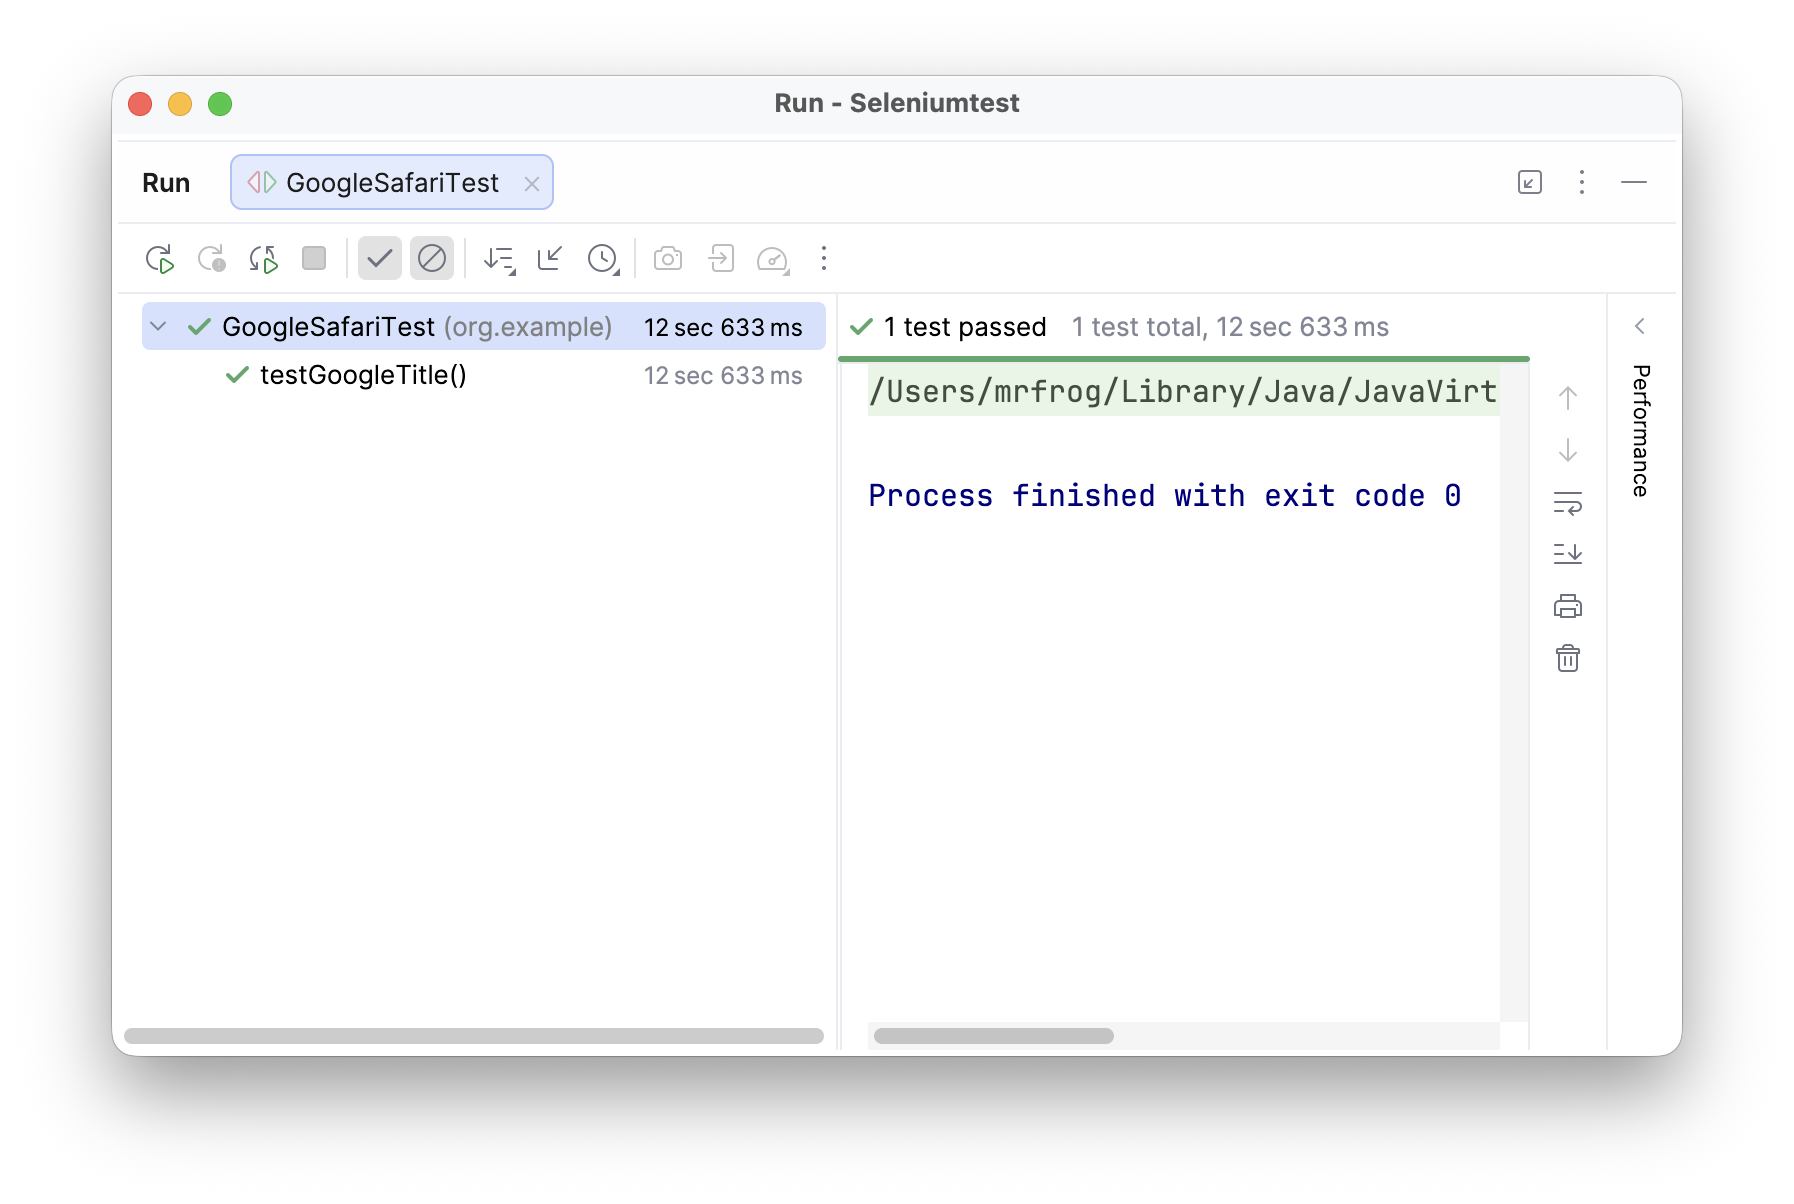
\includegraphics[width=0.9\textwidth]{screenshot step/latihan.png}
    \caption{Hasil Eksekusi Test GoogleSafariTest}
\end{figure}
\newpage
%----------------------------------------------------------------------
\section{Tugas}
%----------------------------------------------------------------------

Berikut adalah penjelasan dan tahap praktikum untuk pembuatan dan eksekusi \textit{Automated Testing} terhadap interaksi aplikasi spesifik, yakni pendaftaran dan verifikasi autentikasi portal SauceDemo.

\subsection{Pengujian Login SauceDemo Sederhana}
Pada bagian ini, kita akan membuat kelas \texttt{SauceDemoLoginTest} untuk memverifikasi proses \textit{login} untuk \textit{standard user} pada situs SauceDemo.

\subsubsection*{1. Mendefinisikan Package dan Import}
Langkah pertama adalah mendefinisikan nama \textit{package} dan melakukan \textit{import library} yang dibutuhkan, seperti \textit{library} dari \textit{framework} pengujian (JUnit 5) dan \textit{library} Selenium WebDriver:

\begin{lstlisting}[style=javastyle, caption=Import Dependencies]
package org.example;

import org.junit.jupiter.api.AfterEach;
import org.junit.jupiter.api.BeforeEach;
import org.junit.jupiter.api.Test;
import org.openqa.selenium.By;
import org.openqa.selenium.WebDriver;
import org.openqa.selenium.WebElement;
import org.openqa.selenium.safari.SafariDriver;

import static org.junit.jupiter.api.Assertions.assertEquals;
\end{lstlisting}

\subsubsection*{2. Persiapan WebDriver (Setup)}
Selanjutnya, kita mendefinisikan kelas pengujian dan melakukan persiapan (\textit{setup}) awal menggunakan anotasi \texttt{@BeforeEach}. Fungsi ini akan dieksekusi sebelum setiap \textit{test method} untuk melakukan inisialisasi \textit{browser} yang akan kita gunakan (dalam hal ini menggunakan \texttt{SafariDriver}).

\begin{lstlisting}[style=javastyle, caption=Inisialisasi Kelas dan Setup WebDriver]
public class SauceDemoLoginTest {

    private WebDriver driver;

    @BeforeEach
    public void setUp() {
        driver = new SafariDriver();
    }
\end{lstlisting}

\subsubsection*{3. Skenario Pengujian Login (Test)}
Tahap ini merupakan \textit{core} pengujian, menggunakan anotasi \texttt{@Test}. WebDriver akan diinstruksikan untuk membuka halaman web (menggunakan \texttt{driver.get()}), mencari elemen berdasarkan ID (menggunakan \texttt{driver.findElement(By.id())}), lalu melakukan interaksi masukan berupa pengetikan \textit{keys} dan klik. Pada akhirnya \textit{assertion} memastikan bahwa halaman yang terbuka setelah proses *login* adalah halaman \textit{inventory}.

\begin{lstlisting}[style=javastyle, caption=Test Method Login Sederhana]
    @Test
    public void testLogin() {
        driver.get("https://www.saucedemo.com/");

        WebElement usernameInput = driver.findElement(By.id("user-name"));
        usernameInput.sendKeys("standard_user");

        WebElement passwordInput = driver.findElement(By.id("password"));
        passwordInput.sendKeys("secret_sauce");

        WebElement loginButton = driver.findElement(By.id("login-button"));
        loginButton.click();

        String currentUrl = driver.getCurrentUrl();
        assertEquals("https://www.saucedemo.com/inventory.html", currentUrl);
    }
\end{lstlisting}

\subsubsection*{4. Membersihkan WebDriver (Teardown)}
Bagian terakhir menggunakan anotasi \texttt{@AfterEach} bertujuan menutup sesi \textit{browser} untuk menghemat \textit{resource} sistem setiap kali sekuens pengujian dari suatu \textit{test case} telah selesai dilaksanakan:

\begin{lstlisting}[style=javastyle, caption=Penutupan Sesi Browser]
    @AfterEach
    public void tearDown() {
        if (driver != null) {
            driver.quit();
        }
    }
}
\end{lstlisting}

\subsubsection*{Hasil Test}
Berikut dilampirkan tangkapan layar sebagai \textit{output} yang membuktikan eksekusi \textit{Automated Testing} telah berjalan dan berhasil mencapai (\textit{passed}) skenario uji tersebut.

\begin{figure}[H]
    \centering
    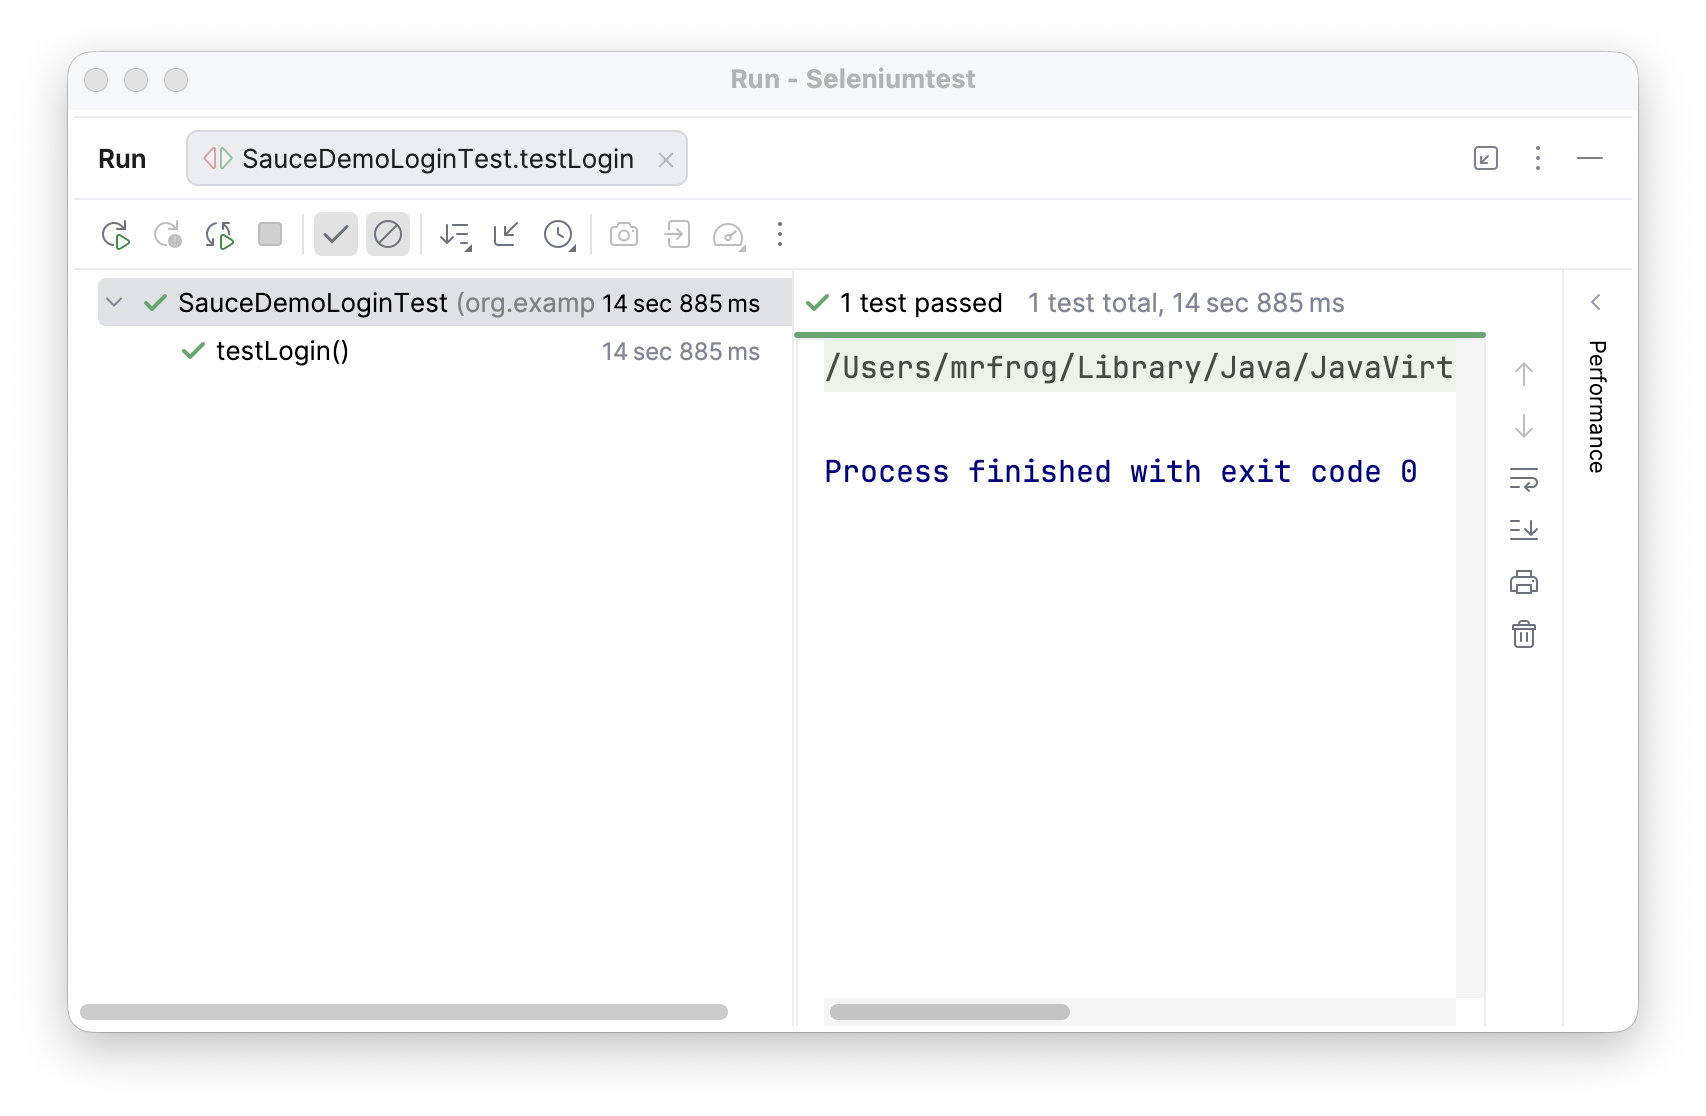
\includegraphics[width=0.9\textwidth]{screenshot step/testlogin.png} \\[0.5cm]
    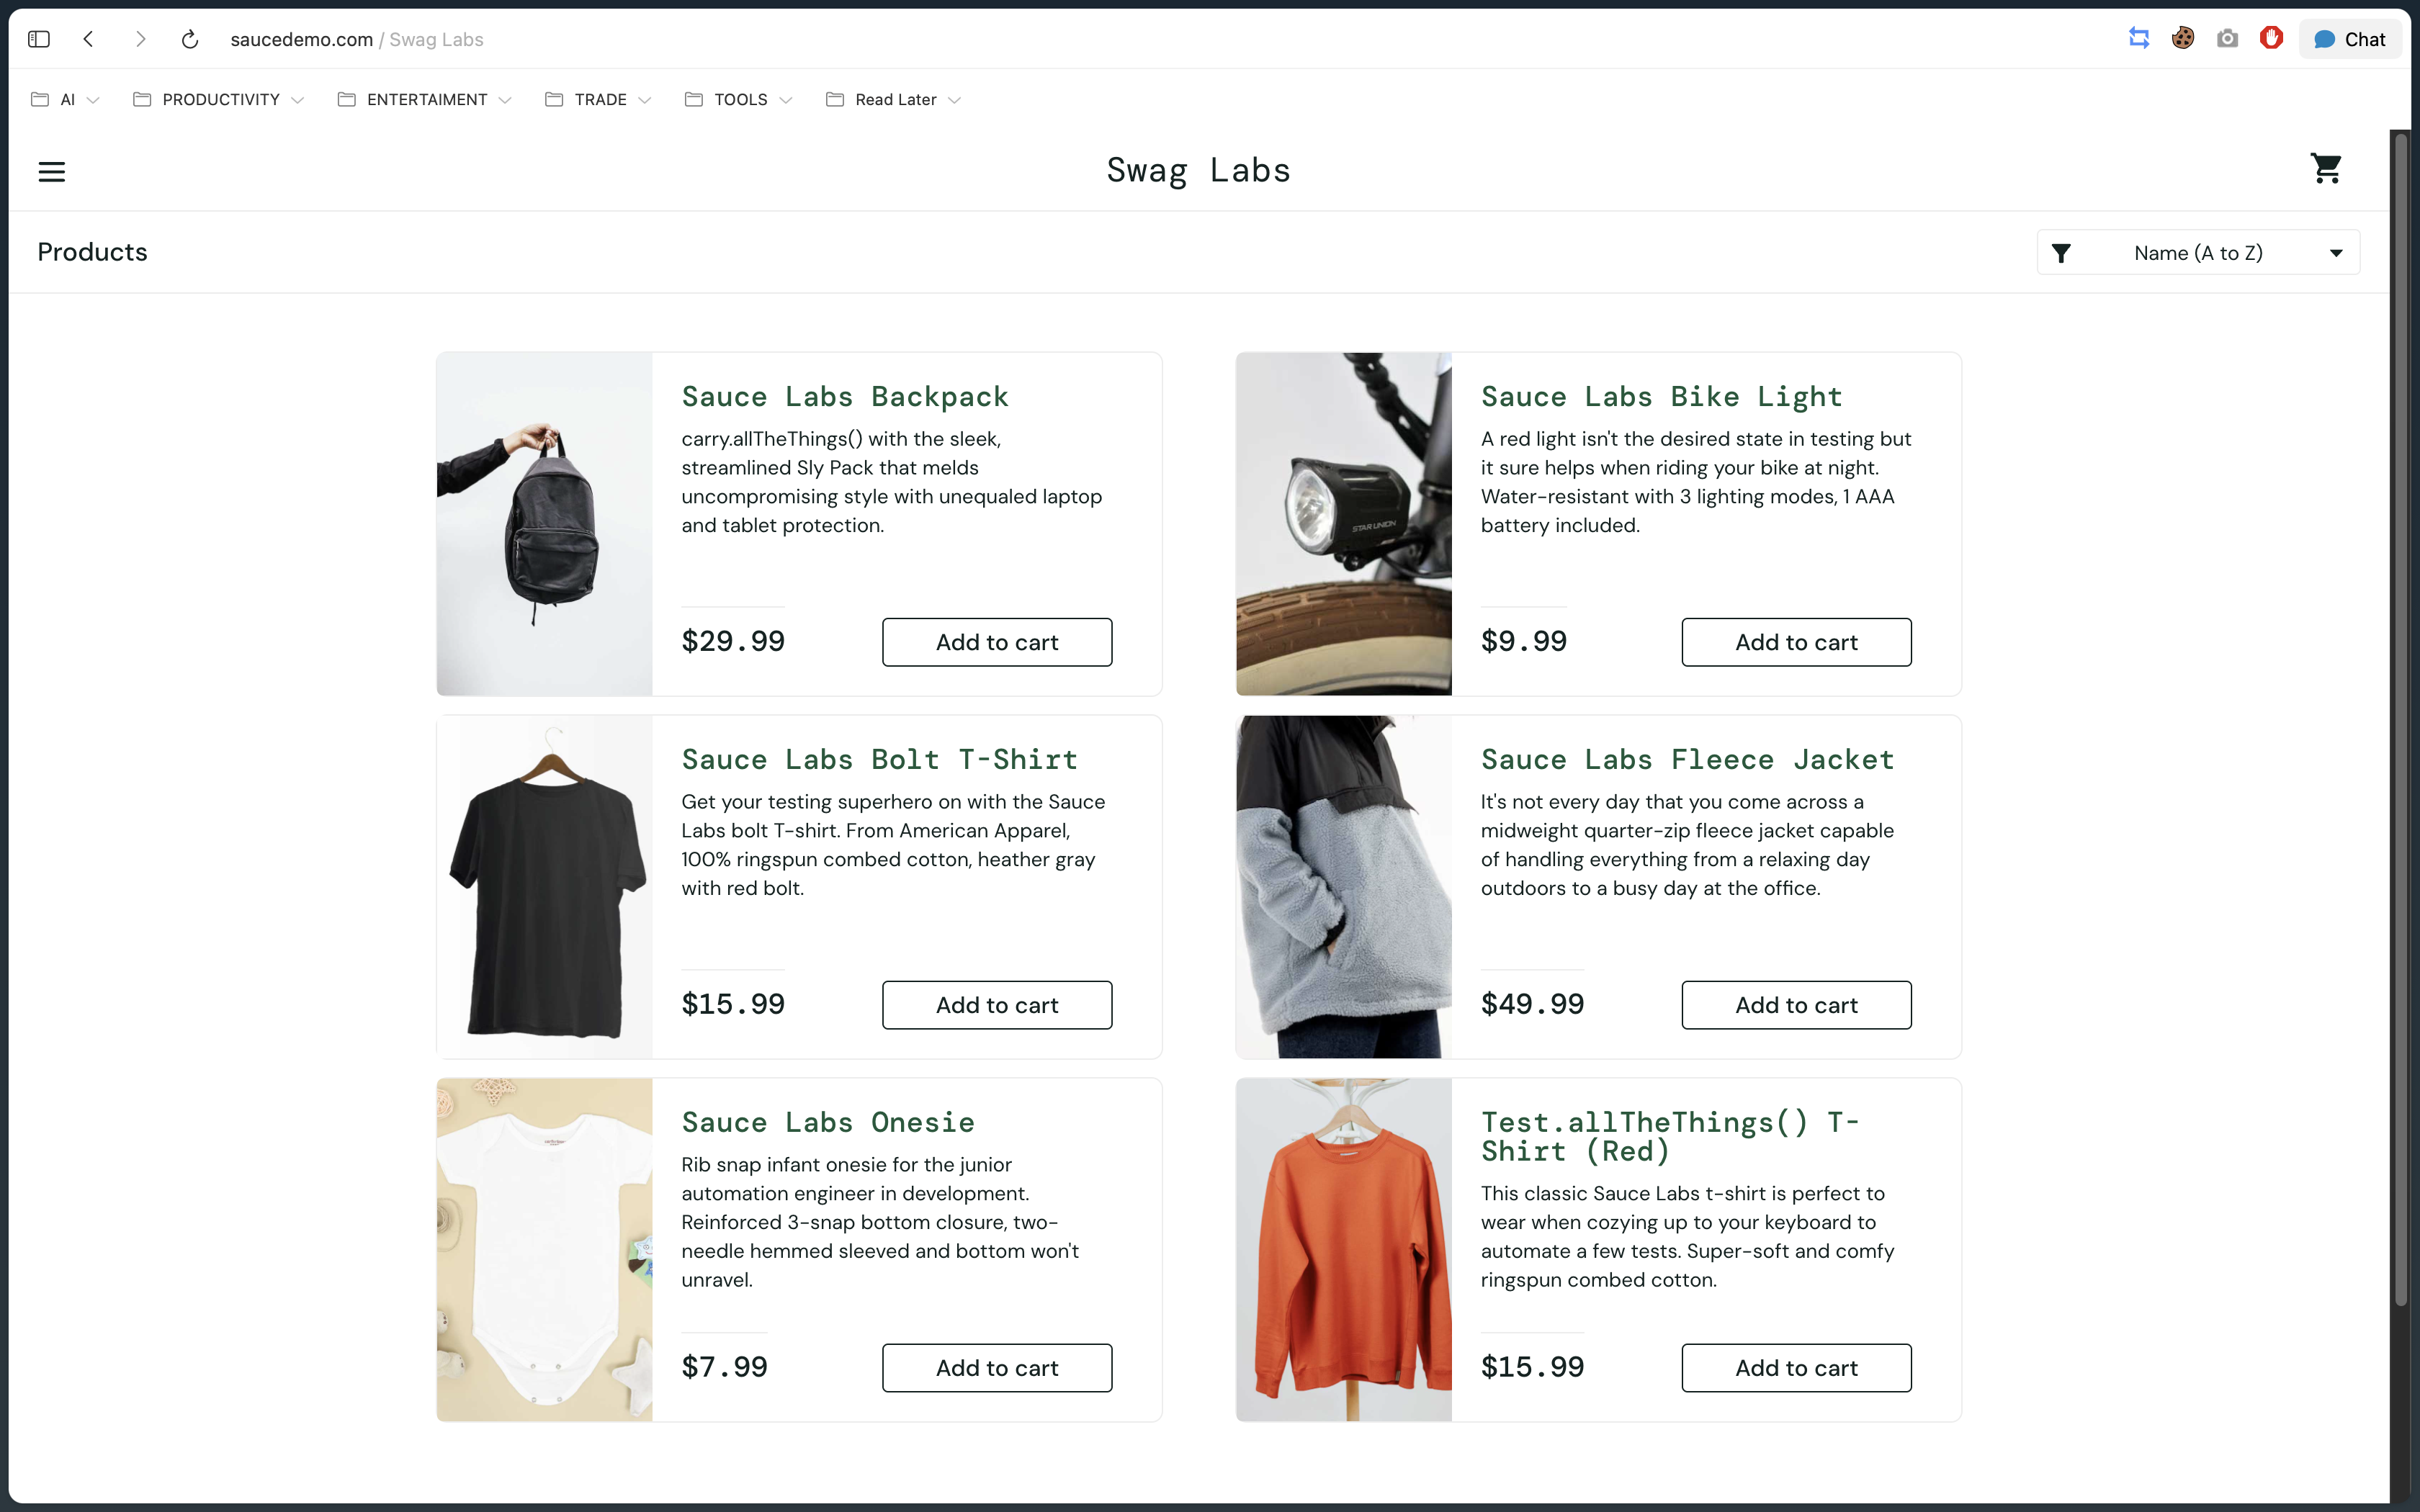
\includegraphics[width=0.9\textwidth]{screenshot step/sauceinventory.png}
    \caption{Hasil Eksekusi Test Login SauceDemo (Test Runner dan Tampilan Browser Output)}
\end{figure}

\subsection{Pengujian Skenario Lengkap Pengguna SauceDemo}
Berikut adalah pengujian yang lebih ekstensif untuk berbagai jenis tipe pengguna (\texttt{locked\_out\_user}, \texttt{problem\_user}, \texttt{performance\_glitch\_user}, dan lainnya) yang membutuhkan \textit{WebDriverWait} untuk mencegah error karena \textit{loading} elemen web.

\subsubsection*{1. Import Library dan Konfigurasi Awal}
Kita menambahkan paket tambahan seperti \texttt{WebDriverWait} maupun \texttt{ExpectedConditions} untuk memfasilitasi penungguan eksplisit ({\textit{Explicit Wait}}).

\begin{lstlisting}[style=javastyle, caption=Import dan Setup Skenario Lengkap]
package org.example;

import org.junit.jupiter.api.AfterEach;
import org.junit.jupiter.api.BeforeEach;
import org.junit.jupiter.api.Test;
import org.openqa.selenium.By;
import org.openqa.selenium.WebDriver;
import org.openqa.selenium.WebElement;
import org.openqa.selenium.safari.SafariDriver;
import org.openqa.selenium.support.ui.ExpectedConditions;
import org.openqa.selenium.support.ui.WebDriverWait;

import java.time.Duration;

import static org.junit.jupiter.api.Assertions.assertEquals;
import static org.junit.jupiter.api.Assertions.assertTrue;

public class SauceDemoAllUsersLoginTest {

    private WebDriver driver;
    private WebDriverWait wait;

    @BeforeEach
    public void setUp() {
        driver = new SafariDriver();
        wait = new WebDriverWait(driver, Duration.ofSeconds(10));
    }
\end{lstlisting}

\subsubsection*{2. Pembuatan Helper Method Login}
Alih-alih menulis sintaks Selenium identik di setiap skenario \textit{user}, kita mengelompokkannya dalam sebuah \textit{method helper} bernama \texttt{login} agar perancangan \textit{Test Case} menjadi lebih rapi dan ringkas (\textit{reusable step}).

\begin{lstlisting}[style=javastyle, caption=Method Helper Interaksi Login]
    private void login(String username, String password) {
        driver.get("https://www.saucedemo.com/");
        driver.findElement(By.id("user-name")).sendKeys(username);
        driver.findElement(By.id("password")).sendKeys(password);
        driver.findElement(By.id("login-button")).click();
    }
\end{lstlisting}
\newpage
\subsubsection*{3. Test Case Standar dan Blocked User}
Pengujian di bawah ini dilakukan berturut-turut untuk validasi \textit{standard\_user} yang seharusnya sukses (diarahkan ke \texttt{/inventory.html}) serta validasi \textit{locked\_out\_user} yang akan memunculkan pesan \textit{error} khusus dan tidak mengubah URL.

\begin{lstlisting}[style=javastyle, caption=Pengujian Standard dan Blocked User]
    @Test
    public void testStandardUserLogin() {
        login("standard_user", "secret_sauce");
        wait.until(ExpectedConditions.urlToBe("https://www.saucedemo.com/inventory.html"));
        assertEquals("https://www.saucedemo.com/inventory.html", driver.getCurrentUrl());
    }

    @Test
    public void testLockedOutUserLogin() {
        login("locked_out_user", "secret_sauce");
        WebElement errorElement = wait.until(ExpectedConditions.visibilityOfElementLocated(By.cssSelector("h3[data-test='error']")));
        assertTrue(errorElement.getText().contains("Epic sadface: Sorry, this user has been locked out."));
        assertEquals("https://www.saucedemo.com/", driver.getCurrentUrl());
    }
\end{lstlisting}

\subsubsection*{4. Uji Lanjutan dan Teardown}
Sama halnya dengan kelas login dasar, setelah semua \textit{test method} dijalankan, kita perlu menutup \textit{driver browser}.

\begin{lstlisting}[style=javastyle, caption=Pengujian Tambahan dan Akhir Siklus]
    @Test
    public void testProblemUserLogin() {
        login("problem_user", "secret_sauce");
        wait.until(ExpectedConditions.urlToBe("https://www.saucedemo.com/inventory.html"));
        assertEquals("https://www.saucedemo.com/inventory.html", driver.getCurrentUrl());
    }

    // Beberapa test lain untuk performance_glitch_user, error_user, dan visual_user juga berhasil diuji...

    @AfterEach
    public void tearDown() {
        if (driver != null) {
            driver.quit();
        }
    }
}
\end{lstlisting}

\subsubsection*{Hasil Test}
Sama halnya dengan kelas sebelumnya, berikut kami tampilkan hasil \textit{run} atau eksekusi *Test Suite* yang menandakan skenario berhasil dilakukan.

\begin{figure}[H]
    \centering
    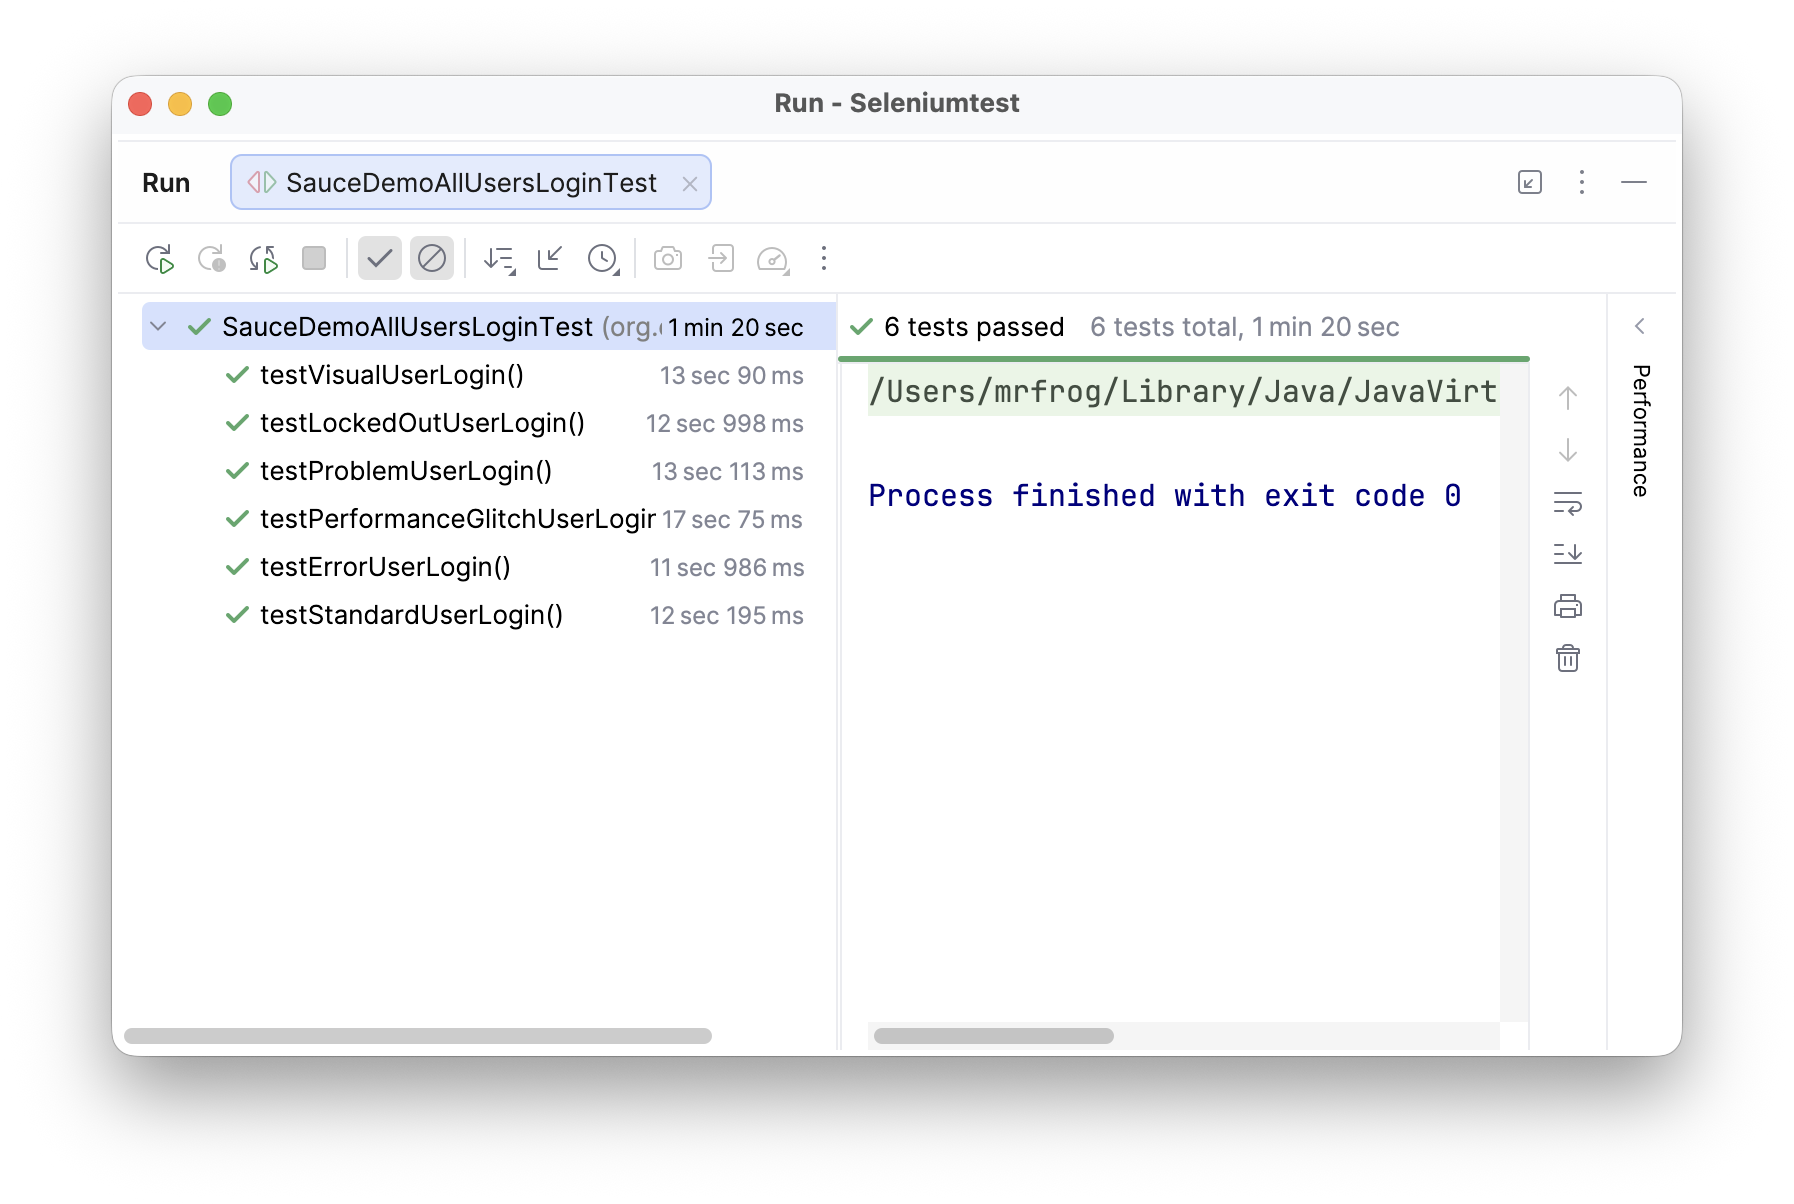
\includegraphics[width=0.9\textwidth]{screenshot step/testalluser.png} \\[0.5cm]
    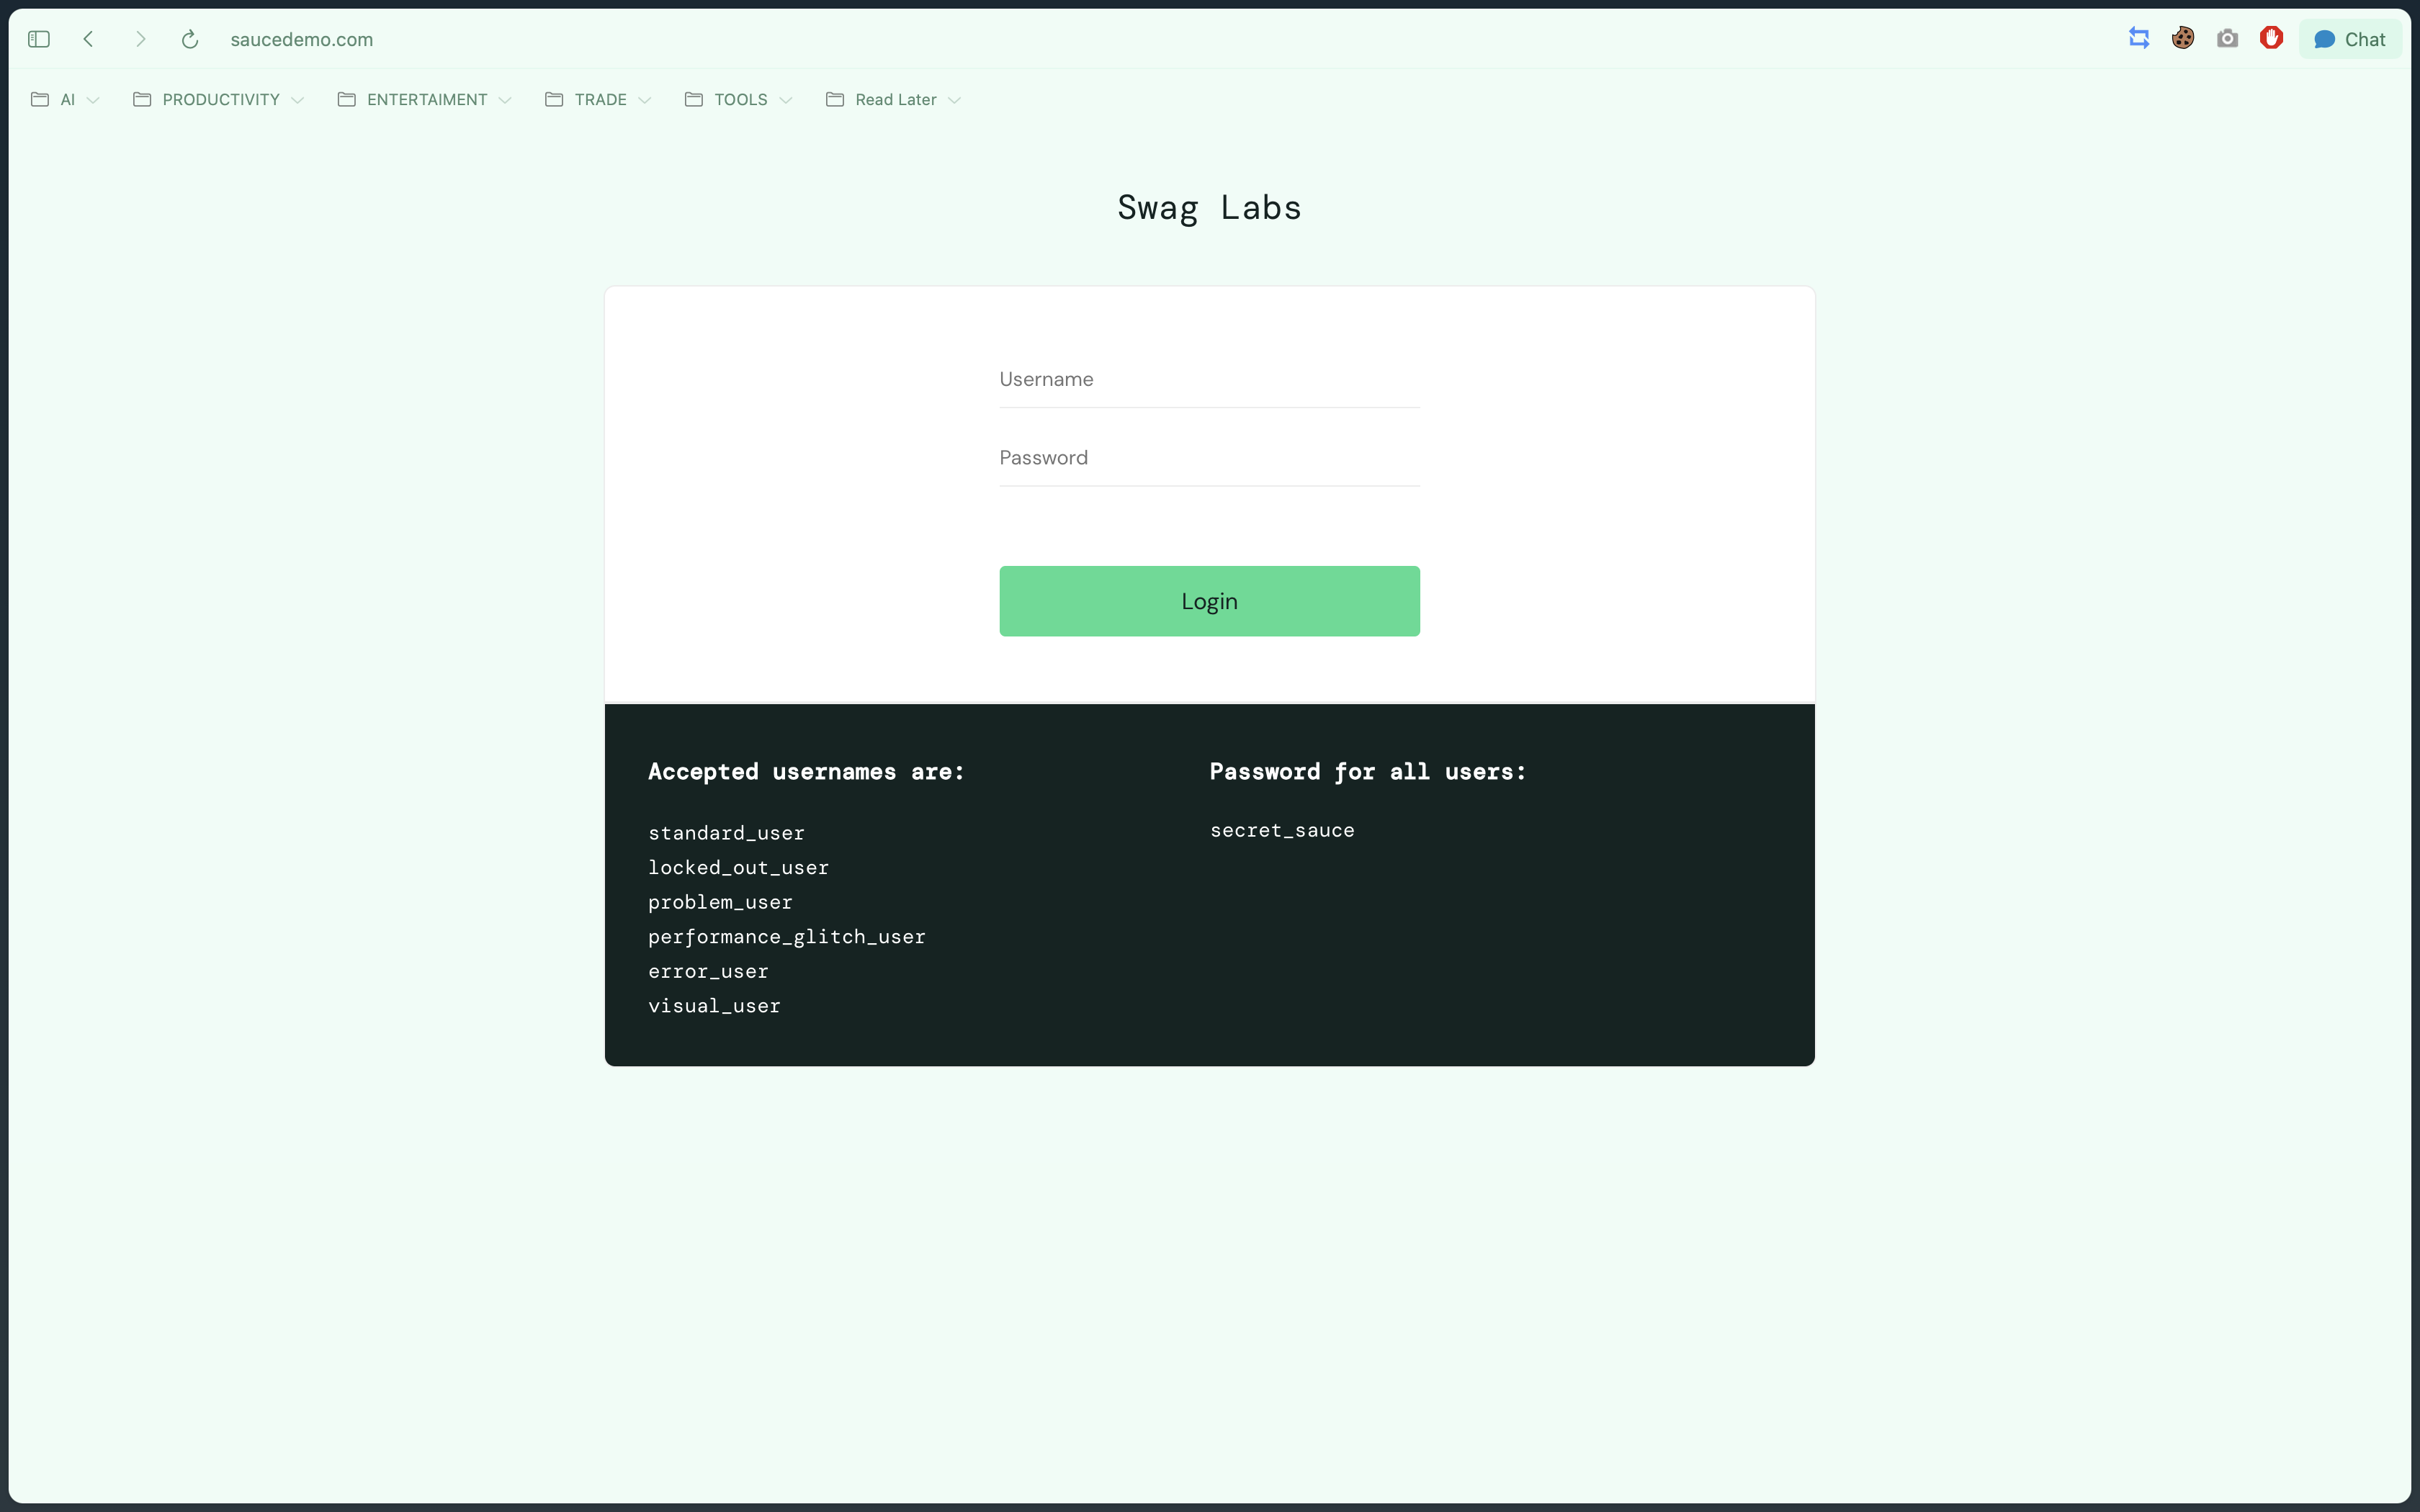
\includegraphics[width=0.9\textwidth]{screenshot step/loginsaucedemo.png}
    \caption{Hasil Eksekusi Test Skenario Seluruh Pengguna (Test Runner dan Kondisi URL Hasil Tes)}
\end{figure}

% \chapter{Resources}
% %======================================================================

\begin{center}
    \url{https://github.com/januarsyah901/PPPL/tree/9d622d374dcf5c9e04c560607ba4e59049f3681a/Pertemuan%207}
\end{center}

\clearpage

%======================================================================
\chapter{Kesimpulan}
%======================================================================

Berdasarkan praktikum yang telah dilakukan, dapat disimpulkan bahwa penggunaan \textit{kakas bantu} seperti Selenium WebDriver sangat mempermudah pembuatan \textit{automated testing} atau pengujian otomatis antarmuka pada suatu aplikasi secara terstruktur. Pengujian \textit{login} pada website \texttt{SauceDemo} dengan menggunakan berbagai \textit{user} telah berhasil diotomatisasi secara rinci. 

Selain itu, pendokumentasian skrip pengujian berbasis \textit{Java} serta JUnit telah menunjukkan bagaimana \textit{webdriver} diinstansiasi, dinavigasi mencari \textit{element} dan divalidasi dengan struktur kode secara langsung. Ini sangat menghemat waktu dibandingkan dengan menguji suatu \textit{form login} dan interaksi-interaksi web secara manual berulang-ulang, menstimulasi produktivitas untuk QA (Quality Assurance) serta \textit{Developer} pada tahap-tahap integrasi perangkat lunak nantinya.

% \clearpage
% \addcontentsline{toc}{chapter}{Daftar Pustaka}
% \renewcommand{\bibname}{Daftar Pustaka}

% \begin{thebibliography}{99}
%     \bibitem{mockito} Mockito Project, ``Mockito --- tasty mocking framework for unit tests in Java''. [Online]. Tersedia: \url{https://site.mockito.org/}.
%     \bibitem{junit5} JUnit Team, ``JUnit 5 User Guide''. [Online]. Tersedia: \url{https://junit.org/junit5/docs/current/user-guide/}.
%     \bibitem{fowler-mocks} Martin Fowler, ``Mocks Aren't Stubs'', 2007. [Online]. Tersedia: \url{https://martinfowler.com/articles/mocksArentStubs.html}.
% \end{thebibliography}

\end{document}
